%%%%%%%%%%%%%%%%%%%%%%%%%%%%%%%%%%%%%%%%%%%%%%%%%%%%%%%%%%%%%%%%%%%%
% This is a thesis template for Gebze Technical University.
%
% Please only edit the areas proceeded by a comment starting with %%
% otherwise the template may be broken.
%
% This file is only to be used for editing the general fields
% and inputting the body of the thesis in the designated areas.
% Please write the body of the thesis in separate files, and input
% them as shown in the comment preceding the area.
%
% Created in Aug 2021 by Usama Derbashi.
%%%%%%%%%%%%%%%%%%%%%%%%%%%%%%%%%%%%%%%%%%%%%%%%%%%%%%%%%%%%%%%%%%%%
\documentclass[12pt]{report}


% Language and typeset setting
\usepackage[english]{babel}
\usepackage[a4paper,top=25mm,bottom=25mm,left=40mm,right=25mm]{geometry}
\usepackage[onehalfspacing]{setspace}
\usepackage{algorithm, algpseudocode}
\usepackage{indentfirst}
\setlength{\parindent}{1cm}
\setlength{\abovecaptionskip}{12pt plus 0pt minus 0pt}
\setlength{\belowcaptionskip}{12pt plus 0pt minus 0pt}
\setlength{\textfloatsep}{18.0pt plus 0.0pt minus 0.0pt}
\setlength{\floatsep}{18.0pt plus 0.0pt minus 0.0pt}
\setlength{\intextsep}{18.0pt plus 0.0pt minus 0.0pt}
\setlength{\skip\footins}{18.0pt plus 0.0pt minus 0.0pt}

% Core packages and settings
\usepackage[colorlinks=false]{hyperref}
\usepackage{amsmath}

\usepackage{titlesec} %setting the titles of chapters and sections
\setcounter{secnumdepth}{4}
\setcounter{tocdepth}{4}
\titleformat{\chapter}[hang]{\normalfont\bfseries\MakeUppercase}{}{0pt}{\LARGE\thechapter. }
\titleformat{\section}[hang]{\normalfont\bfseries}{}{0pt}{\Large\thesection. }
\titleformat{\subsection}[hang]{\normalfont\bfseries}{}{0pt}{\large\thesubsection. }
\titleformat{\subsubsection}[hang]{\normalfont\bfseries}{}{0pt}{\large\thesubsubsection. }
\titlespacing*{\chapter}{0pt}{0pt}{18pt}
\titlespacing*{\section}{0pt}{18pt}{18pt}
\titlespacing*{\subsection}{0pt}{18pt}{18pt}
\titlespacing*{\subsubsection}{0pt}{18pt}{18pt}

\usepackage{graphicx}
\graphicspath{{./Imgs/}} %pointing the directory of images

\usepackage{fancyhdr} % setting footers
\usepackage{etoolbox} 
\renewcommand{\headrulewidth}{0pt}
\patchcmd{\chapter}{\thispagestyle{plain}}{\thispagestyle{fancy}}{}{}
\pagestyle{fancy}
\fancyhf{}
\fancyfoot[C]{\fontsize{11pt}{11pt}\thepage}

\usepackage[style=ieee]{biblatex}
\addbibresource{refs.bib}
\usepackage{csquotes}% Needed for babel(in biblatex)

\usepackage[bottom, perpage]{footmisc}%% amkes footnotes at the bottom

\usepackage{GTUThesis}


% Additional packages if needed
%% For the sake of not messing the template add them here
\usepackage{lipsum}


% Important information
%% Make sure to enter all the info below
\title{Active Planning for Multiple UAV Localization}
\author{İBRAHİM Barış Uysal}
\faculty{Faculty of Engineering}
\department{Computer Engineering Department}
\supervisor{Assist. Prof. Yakup GENÇ}
\theyear{2025}


\begin{document}

%Front Matter
\pagenumbering{roman} %start with roman numbering 
\projecttitlepageenglish
\maketitle
\setcounter{page}{3} %the first two title pages are not counted so this is a buffer
\begin{outertitles} % makes titles centred

%% below enter as follows 
%% {DATE_OF_DEMO}{JURY}
%% Note that JURY should be comma separated
\makejury{15/01/2025}{Prof. Yusuf Sinan AKGÜL}
\chapter*{Abstract}
\addcontentsline{toc}{chapter}{Abstract}

%% Edit below this line
The accurate localization of unmanned aerial vehicles (UAVs) is crucial for various applications, including surveillance, disaster response, and environmental monitoring. However, localization is often challenged by GPS inaccuracies, especially in complex environments. This project presents a novel approach to localizing a target UAV by employing an observer UAV equipped with a stationary camera. The observer UAV captures the target UAV's trajectory through video footage, allowing for the estimation of its local coordinates without direct GPS dependence.

A simulation environment was developed to emulate the flight of both UAVs under realistic GPS noise conditions. A convolutional neural network (CNN) model was trained using datasets generated from the simulation, enabling precise prediction of the target UAV’s position based solely on visual data. The model was then deployed within the simulation to evaluate its performance in real-time localization tasks.

The results demonstrate that the proposed method achieves reliable localization accuracy despite significant GPS noise, serving as a good example in the field of vision-based localization systems for UAV operations. 

%% Until here
\vfill
%% Edit after {Keywords:}
\textbf{Keywords:} UAV Localization, Active Planning, GPS Noise, Convolutional Neural Network, Simulation Environment.
\clearpage
\chapter*{Özet}
\addcontentsline{toc}{chapter}{Özet}

%% Edit below this line

İnsansız hava araçlarının (İHA) doğru bir şekilde konumlandırılması, gözetim, afet müdahalesi ve çevre izleme gibi çeşitli uygulamalar için büyük önem taşımaktadır. Ancak, karmaşık ortamlarda GPS hataları nedeniyle konumlandırma genellikle zorlu bir hale gelmektedir. Bu proje, hedef bir İHA'nın yerel koordinatlarını, sabit bir kamerayla donatılmış bir gözlemci İHA kullanarak konumlandırmak için yenilikçi bir yaklaşım sunmaktadır. Gözlemci İHA, hedef İHA'nın uçuş rotasını video görüntüleri aracılığıyla kaydederek, doğrudan GPS'e bağımlı olmadan yerel koordinatlarının tahmin edilmesini sağlamaktadır.

Her iki İHA'nın uçuşunu gerçekçi GPS gürültü koşulları altında simüle etmek için bir simülasyon ortamı geliştirilmiştir. Konvolüsyonel sinir ağı (CNN) modeli, simülasyondan üretilen veri setleri kullanılarak eğitilmiş ve sadece görsel verilere dayanarak hedef İHA'nın konumunu hassas bir şekilde tahmin edebilmiştir. Model, gerçek zamanlı konumlandırma görevlerinde performansını değerlendirmek amacıyla simülasyon ortamında kullanılmıştır.

Elde edilen sonuçlar, önerilen yöntemin önemli GPS gürültüsüne rağmen güvenilir konumlandırma doğruluğu sağladığını göstermektedir. 

%% Until here
\vfill
%% Edit after {Anahtar Kelimeler:}
\textbf{Anahtar Kelimeler:} İHA Konumlandırma, Aktif Planlama, GPS Gürültüsü, Evrişimsel Sinir Ağı, Simülasyon Ortamı.







\clearpage
\chapter*{Acknowledgement}
\addcontentsline{toc}{chapter}{Acknowledgement}

%% Edit below this line
I would like to express my sincere gratitude to my advisor, Yakup Genç, for their guidance, support, and valuable insights throughout this project. Their expertise and constructive feedback have been instrumental in shaping the direction and outcomes of this study. \\
I am especially grateful to my sister, whose support has been a constant source of strength and motivation for me. Her belief in my abilities, her patience and encouragement during difficult times guided me on my academic journey and helped me in my personal growth.
%% Until here
\vspace{1cm}
\begin{flushright}
\textbf{İbrahim Barış Uysal} %% your name here
\end{flushright}
\clearpage
\chapter*{List of Symbols and Abbreviations}
\addcontentsline{toc}{chapter}{List of Symbols and Abbreviations}

\renewcommand{\arraystretch}{1.2} % Adjust row spacing
\setlength{\tabcolsep}{4pt} % Adjust column spacing
\small % Reduce font size
\begin{tabular}{@{}p{3cm}p{0.5cm}p{10cm}@{}}
    \textbf{Symbol or Abbreviation} & : & \textbf{Explanation} \\ \hline
    ReLU & : & Rectified Linear Unit, an activation function that outputs the input if it is positive and zero otherwise. \\
    Tanh & : & Hyperbolic Tangent, an activation function with outputs ranging from -1 to 1. \\
    ELU & : & Exponential Linear Unit, an activation function that allows smoother gradients for negative inputs. \\
    NED & : & North-East-Down, a coordinate system used for defining positions in UAV systems. \\
    UAV & : & Unmanned Aerial Vehicle, commonly referred to as a drone. \\
    MED & : & Mean Euclidean Distance, a metric for measuring the average distance between predicted and actual values. \\
    $\alpha$ & : & A parameter controlling the slope for negative inputs in Leaky ReLU and ELU functions. \\
    GPS & : & Global Positioning System, a satellite-based navigation system. \\
    ML & : & Machine Learning, a field of artificial intelligence focused on enabling systems to learn and improve from experience. \\
    CNN & : & Convolutional Neural Network, a class of deep neural networks, most commonly applied to analyzing visual imagery. \\
    K-Fold & : & A cross-validation technique where data is split into k subsets for training and validation. \\
    Hyperband & : & A method for hyperparameter optimization that dynamically allocates resources to different configurations. \\
\end{tabular}

\clearpage


\tableofcontents
\addcontentsline{toc}{chapter}{Contents}
\clearpage

\listoffigures
\addcontentsline{toc}{chapter}{List of Figures}
\clearpage

\listoftables
\addcontentsline{toc}{chapter}{List of Tables}
\clearpage

\end{outertitles}
\fancyhf{}%reset footer
\fancyfoot[R]{\fontsize{11pt}{11pt}\thepage}%page numbers in the corner
\addtocontents{toc}{\protect\vspace{18pt}}
\pagenumbering{arabic}%turn to arabic numbers

% Mainmatter

%% Only input files, don't write here
%% \input{./Body/Mainmatter/FILE}
\chapter{Introduction}

This project focuses on developing a system to predict target UAV's relative position based on observer UAV. The main goal is to improve the accuracy of localization of UAV.

The system uses a preprocessing pipeline that extracts trajectory information from images captured during UAV movement. These images are processed to create inputs for a prediction model, which also considers  initial UAV positions. The model then predicts the target UAV's relative position.

Testing was conducted in a simulation environment with various conditions, including different noise levels and different inital poisitons. The results showed that the system predicts target UAV's relative position with high accuracy, even in challenging scenarios. The errors between predicted and real trajectories were analyzed to evaluate the performance of the model.

This project demonstrates a practical approach to using prediction models for UAV trajectory tracking. It can be useful in applications such as autonomous navigation and aerial monitoring.


\chapter{Method}


\section{Simulation Environment}

To develop and test the proposed UAV localization system, a simulation environment was prepared using Gazebo, ROS2, and ArduCopter. This simulation setup emulates realistic UAV flight scenarios under GPS noise, allowing for data collection and model evaluation.

\subsection{Tools and Frameworks}
\begin{itemize}
    \item \textbf{Gazebo}: Used as the primary simulation environment to model the physical world, including terrain, environmental features, and UAV dynamics.
    \item \textbf{ROS2 (Robot Operating System 2)}: Served as the middleware for communication between the UAV models, sensors, and control algorithms.
    \item \textbf{ArduCopter}: Employed as the flight control firmware to simulate UAV behaviors such as trajectory following and hovering.
    \item \textbf{pymavlink}: Used for establishing communication between the UAVs, enabling the transmission of MAVLink messages to control UAVs.
\end{itemize}
To enable multi-UAV simulation in the Gazebo and ROS2 environment, several custom modifications were implemented, as the default simulation setups primarily support single-UAV scenarios. The Gazebo world file was updated to include two UAVs: an observer UAV and a target UAV, with appropriate initial relative positions and parameters to ensure smooth operation. To facilitate easy detection by the observer UAV, the target UAV was visually customized by painting it red, improving visibility in the observer UAV's camera. Separate ROS2 topics were created for both UAVs, enabling communication and data exchange, including GPS data, camera feeds, trajectory updates, and control commands. These modifications were essential for achieving independent operation and monitoring of each UAV within the simulation environment. Since built-in support for multi-UAV operations is not provided in the default setups, these changes were manually implemented to enable testing of the proposed localization system. Figure~\ref{fig:gazebo_world} shows the modified Gazebo environment with the two UAVs, while Figure~\ref{fig:observer_camera} presents the observer UAV’s camera view.
\begin{figure}[H]
    \centering
    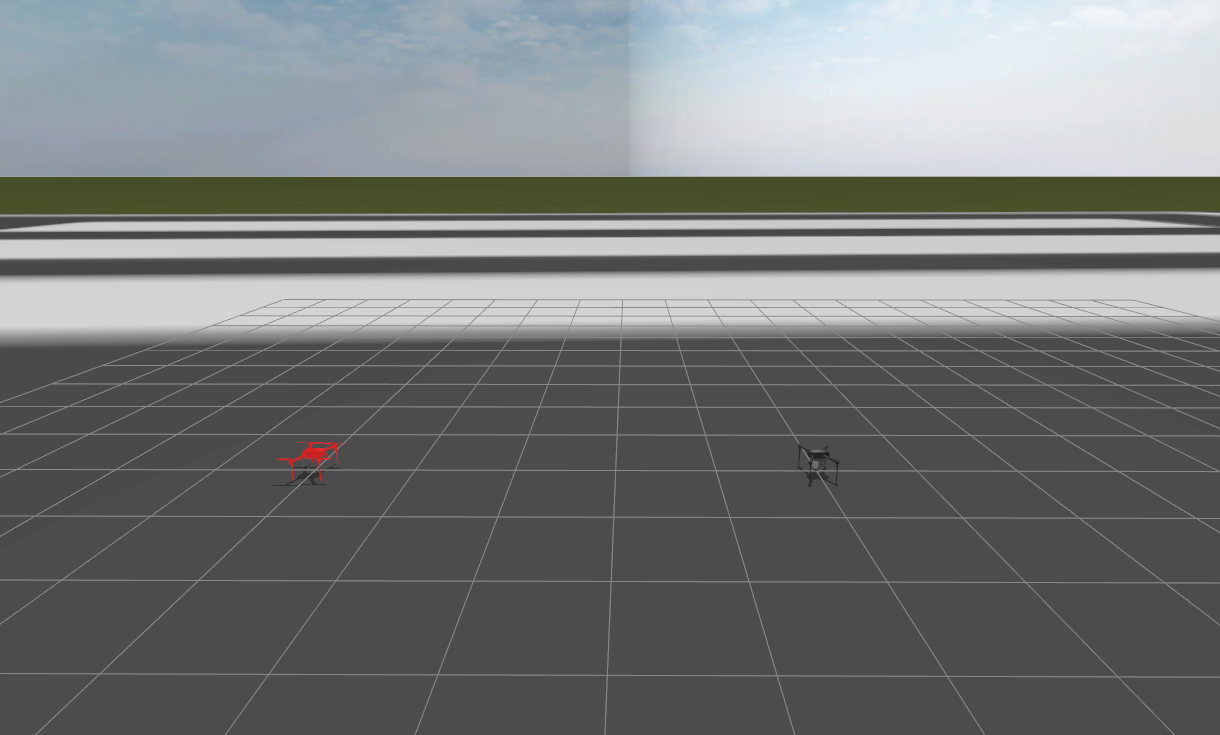
\includegraphics[width=0.8\textwidth]{Imgs/gazebo.png}
    \caption{The modified Gazebo environment with the observer UAV and the red-painted target UAV.}
    \label{fig:gazebo_world}
\end{figure}

\begin{figure}[H]
    \centering
    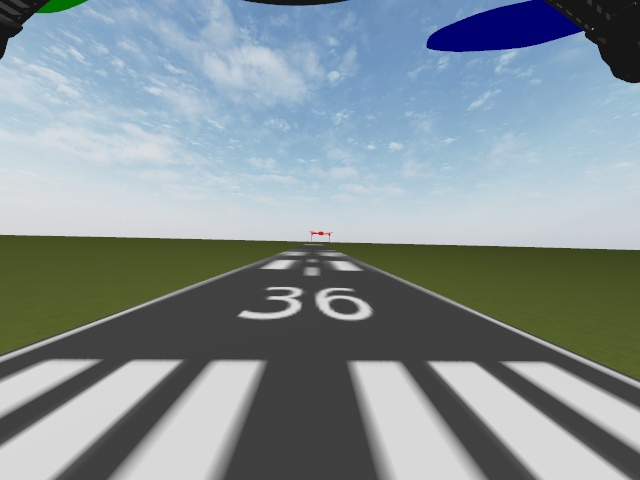
\includegraphics[width=0.8\textwidth]{Imgs/observer_camera.jpg}
    \caption{Camera view from the observer UAV.}
    \label{fig:observer_camera}
\end{figure}
\subsection{ROS2 Integration}

The integration of \textbf{ROS2} facilitated real-time communication between the Gazebo simulation environment and the control algorithms. The key components of the integration are described below:

\begin{itemize}
    \item \textbf{Topic Communication}: ROS2 topics were used to enable data exchange between various components in the simulation. 
    \item \textbf{Control Nodes}: Custom ROS2 nodes were developed to manage the UAV’s trajectory and synchronize data collection. These nodes ensured proper coordination between the UAV models and the simulation environment.
    \item \textbf{TF Frames}: Transform frames (\texttt{tf2}) were set up to maintain accurate alignment of the UAVs within the simulated world. This ensured consistency between the physical positions of the UAVs and their virtual representations.
\end{itemize}

This integration ensured seamless communication and coordination in the simulation, enabling accurate data collection and reliable testing of the proposed localization system.

\subsection{Simulating GPS Noise}

To replicate GPS noise, Gaussian noise was applied to the target and observer UAV’s GPS data. The simulation environment utilized the Gazebo satellite sensor topic to retrieve raw GPS coordinates. A ROS2 node was implemented to apply controlled Gaussian noise to the data. The GPS sensor data was adjusted by adding Gaussian noise scaled by the specified noise level.
The GPS noise was applied to the latitude, longitude, and altitude values using the following calculations:

\begin{align*}
    \text{Latitude} &= \text{round}(\text{Latitude}_{\text{raw}} + \mathcal{N}(0, \sigma_{\text{lat}}), 7) \times 10^7, \\
    \text{Longitude} &= \text{round}(\text{Longitude}_{\text{raw}} + \mathcal{N}(0, \sigma_{\text{lon}}), 7) \times 10^7, \\
    \text{Altitude} &= \text{Altitude}_{\text{raw}} + \mathcal{N}(0, \sigma_{\text{alt}}),
\end{align*}

where:
\begin{itemize}
    \item \(\mathcal{N}(0, \sigma)\) represents Gaussian noise with a mean of 0 and a standard deviation of \(\sigma\),
    \item \(\sigma_{\text{lat}} = \text{noise\_level} \times 10^{-6}\) scales the noise for latitude,
    \item \(\sigma_{\text{lon}} = \text{noise\_level} \times 10^{-6}\) scales the noise for longitude,
    \item \(\sigma_{\text{alt}} = \text{noise\_level} \times 0.1\) scales the noise for altitude.
\end{itemize}
\begin{figure}[H]
    \centering
    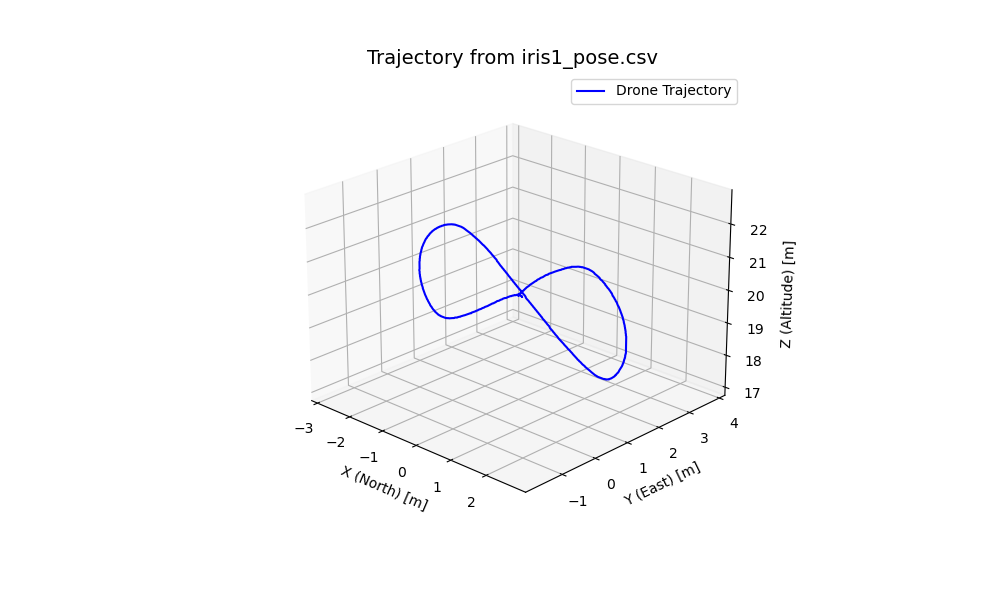
\includegraphics[width=0.8\textwidth]{Imgs/non_noise.png}
    \caption{Trajectory of the UAV without GPS noise.}
    \label{fig:non_noised_trajectory}
\end{figure}

\begin{figure}[H]
    \centering
    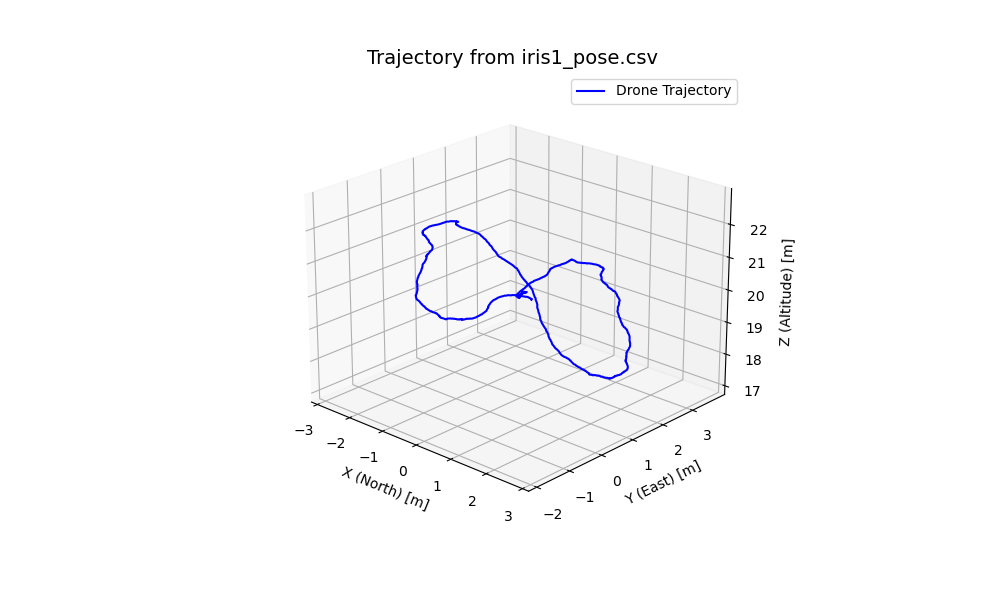
\includegraphics[width=0.8\textwidth]{Imgs/noised_traj.png}
    \caption{Trajectory of the UAV with Gaussian GPS noise applied.}
    \label{fig:noised_trajectory}
\end{figure}


\subsection{Target UAV Trajectory Generation}

The trajectory of the target UAV was designed to follow an eight-shaped path in the body frame and then transformed into the global frame. The mathematical formulation for this process is detailed below:

\subsubsection{ Body Frame Trajectory}
The eight-shaped trajectory in the body frame is parameterized by:
\[
\begin{aligned}
    x_b(\theta) &= L \sin(\theta), \\
    y_b(\theta) &= A \cos(\theta) \sin(\theta), \\
    z_b(\theta) &= 0,
\end{aligned}
\]
where:
\begin{itemize}
    \item \( \theta \) is the angular parameter, uniformly sampled over \([0, 2\pi]\),
    \item \( L \) is the length parameter, controlling the longitudinal dimension,
    \item \( A \) is the amplitude parameter, controlling the lateral dimension.
\end{itemize}

The body frame trajectory is expressed as:
\[
\mathbf{p}_b(\theta) = 
\begin{bmatrix}
    x_b(\theta) \\
    y_b(\theta) \\
    z_b(\theta)
\end{bmatrix}.
\]

\subsubsection{ Global Frame Transformation}
The trajectory is transformed to the global frame through a series of rotations and translations. The total transformation is represented by:
\[
\mathbf{p}_g = \mathbf{R}_\text{total} \mathbf{p}_b + \mathbf{t},
\]
where:
\begin{itemize}
    \item \(\mathbf{R}_\text{total}\) is the total rotation matrix,
    \item \(\mathbf{t} = [t_x, t_y, t_z]^T\) is the translation vector representing the UAV's position in the global frame.
\end{itemize}

\paragraph{ Rotation Matrices}
The total rotation matrix is derived by combining rotations around the X, Y, and Z axes:
\[
\mathbf{R}_\text{total} = \mathbf{R}_z(\psi) \mathbf{R}_y(\theta_y) \mathbf{R}_x(\theta_x),
\]
where:
\[
\mathbf{R}_z(\psi) =
\begin{bmatrix}
    \cos\psi & -\sin\psi & 0 \\
    \sin\psi & \cos\psi & 0 \\
    0 & 0 & 1
\end{bmatrix}, \quad
\mathbf{R}_y(\theta_y) =
\begin{bmatrix}
    \cos\theta_y & 0 & \sin\theta_y \\
    0 & 1 & 0 \\
    -\sin\theta_y & 0 & \cos\theta_y
\end{bmatrix},
\]
\[
\mathbf{R}_x(\theta_x) =
\begin{bmatrix}
    1 & 0 & 0 \\
    0 & \cos\theta_x & -\sin\theta_x \\
    0 & \sin\theta_x & \cos\theta_x
\end{bmatrix}.
\]

\paragraph{ Translation}
The trajectory is translated to the UAV's global position by adding the translation vector:
\[
\mathbf{t} = 
\begin{bmatrix}
    t_x \\
    t_y \\
    t_z
\end{bmatrix}.
\]

\subsubsection{ Final Global Trajectory}
The final global trajectory is given by:
\[
\mathbf{p}_g(\theta) = \mathbf{R}_\text{total}
\begin{bmatrix}
    x_b(\theta) \\
    y_b(\theta) \\
    z_b(\theta)
\end{bmatrix}
+
\begin{bmatrix}
    t_x \\
    t_y \\
    t_z
\end{bmatrix}.
\]

This mathematical model provides a parameterized, flexible framework for generating complex trajectories for the target UAV. An example of the generated trajectory is shown in Figure~\ref{fig:eight_trajectory}.

\begin{figure}[H]
    \centering
    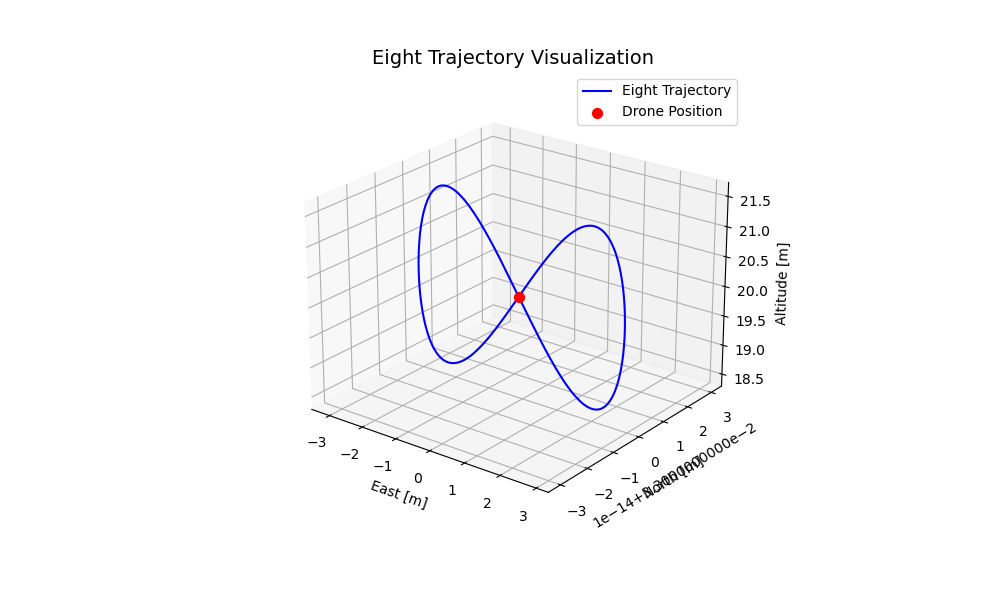
\includegraphics[width=0.8\textwidth]{Imgs/trajectory.png}
    \caption{Example of the eight-shaped trajectory generated for the target UAV.}
    \label{fig:eight_trajectory}
\end{figure}


\section{GUI Integration for Simulation Control}
A custom graphical user interface (GUI) was developed using PyQt5 to provide an interactive control mechanism for managing simulation parameters. The GUI was integrated with the ROS2 node. The GUI includes sliders for adjusting GPS noise levels for both observer and target UAVs. The GUI allows the user to start and stop trajectory recording, capturing the position of target UAV during the simulation. Users can input custom parameters for target UAV trajectory, such as trajectory dimensions, update intervals, and trajectory alignment angles, which are published to ROS2 topics to dynamically modify target UAV trajectory. The GUI displays the predictions of the developed localization model in real-time, alongside the actual positions of the UAV.  Furthermore, the GUI supports visualizing trajectories from the recorded dataset stored in CSV files. Users can load a CSV file containing trajectory data and view a 3D plot of the UAVs paths. The GUI includes features for recording data into CSV files or ROS2 bag files.
An example view of the GUI interface is shown in Figure~\ref{fig:gui_interface}.

\begin{figure}[H]
    \centering
    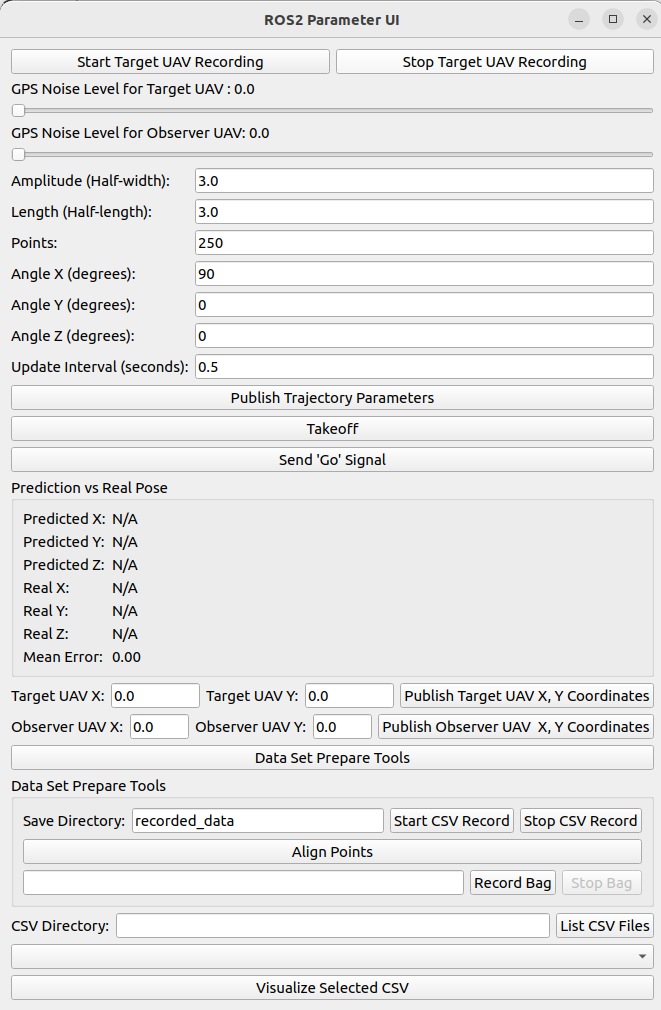
\includegraphics[width=0.4\textwidth]{Imgs/gui.png}
    \caption{Custom GUI developed using PyQt5 for simulation control.}
    \label{fig:gui_interface}
\end{figure}



\section{Dataset Preparation}

The dataset for training and evaluating the localization model was prepared by processing simulation outputs. The steps involved in the preparation are detailed below:

\subsubsection{Data Collection}
Simulation data was recorded as ROS bag files using a custom GUI. These files contained relevant topics such as:
\begin{itemize}
    \item Observer UAV’s local and global locations,
    \item Target UAV’s local and global locations,
    \item GPS (NavSat) data,
    \item Target UAV's trajectory, and
    \item Camera images from the observer UAV.
\end{itemize}

\subsubsection{ Data Processing}
The collected ROS bag files were processed to extract relevant topics and save them in CSV format. The processing steps included:
\begin{itemize}
    \item \textbf{Extracting Locations:} Local, global, and GPS locations of both UAVs were saved as separate CSV files.
    \item \textbf{Image Processing:} Images captured from the observer UAV’s camera were saved and aligned with the corresponding trajectory data based on timestamps (\texttt{Sec} and \texttt{Nanosec} fields). Since the topics were published at different frequencies, synchronization was performed to ensure data consistency.
\end{itemize}

\subsubsection{Trajectory Image Generation}
Using the processed data, images with overlayed target UAV trajectories were generated. The steps included:
\begin{itemize}
    \item \textbf{Target UAV Detection:} The target UAV was detected in the images using a color-based approach, leveraging its distinct red color.
    \item \textbf{Trajectory Overlay:} The trajectory points of the target UAV were overlayed on the images to create a visual representation of the flight path. Outlier points were removed using statistical methods, and the trajectory was resampled for uniformity.
\end{itemize}

\subsubsection{ Final Dataset Creation}
For training and evaluation, the dataset was structured with the following features:
\begin{itemize}
    \item \textbf{Start and End Locations:} The start and end positions of both the observer and target UAVs were extracted and saved.
    \item \textbf{Trajectory Images:} The processed images with overlayed trajectories were included as inputs.
    \item \textbf{Aligned Data:} All data points, including images and locations, were synchronized using timestamps to ensure consistency across the dataset.
\end{itemize}

\subsubsection{ Data Storage}
The final dataset was saved as structured \texttt{.npy} files, containing:
\begin{itemize}
    \item Masked Trajectory image
    \item Start and end positions of both UAVs, and
    \item Supporting metadata for model training and evaluation.
\end{itemize}

This structured dataset provided a robust foundation for developing and testing the UAV localization model. An example of the generated trajectory image is shown in Figure~\ref{fig:trajectory_image}.

\begin{figure}[H]
    \centering
    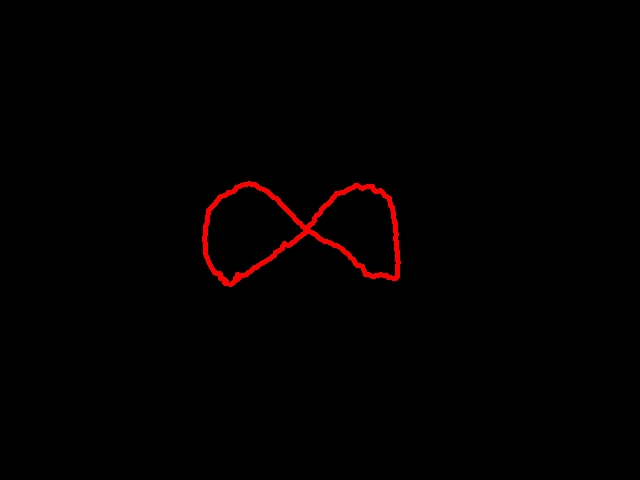
\includegraphics[width=0.5\textwidth]{Imgs/iris1_trajectory_masked.jpg}
    \caption{Example of a generated trajectory image.}
    \label{fig:trajectory_image}
\end{figure}

A total of 60 trajectory simulations were conducted, with the target UAV moving along eight-shaped paths. The starting positions of the trajectories varied along the 
North direction, ranging from 3 to 10 meters, on same GPS noise level.

\section{CNN Model}

The proposed model predicts the final location of a target UAV by processing trajectory images and initial relative location data. It employs a convolutional neural network (CNN) for feature extraction and a regression head for position prediction. The architecture is detailed as follows:

\subsection{Inputs}
The model is designed to handle two types of inputs:
\begin{enumerate}
    \item \textbf{Trajectory Image Input:} A masked image of the UAV’s trajectory, preprocessed to emphasize trajectory points with color-based masking. The image captures the UAV’s path and provides spatial context for predicting the final position.
    \item \textbf{Initial Relative Location Input:} A three-dimensional vector \((x_0, y_0, z_0)\) representing the UAV's starting coordinates differences in observer UAV local NED frame. 
\end{enumerate}

\subsection{Backbone for Feature Extraction}
The trajectory image is processed using a pre-trained \textbf{MobileNetV2} model, which serves as the backbone for feature extraction. MobileNetV2 is a convolutional neural network architecture designed for efficient image processing. Key details include:
\begin{itemize}
    \item \textbf{Pre-Trained Weights:} MobileNetV2 is initialized with ImageNet weights.
    \item \textbf{Global Average Pooling (GAP):} After feature extraction, the spatial dimensions of the feature maps are reduced using a GAP layer, aggregating the extracted features into a fixed-size vector.
\end{itemize}

\subsection{Input Fusion}
The extracted feature vector from the trajectory image is concatenated with the initial relative location vector. 
\subsection{Regression Head}
The regression head processes the fused data to predict the final coordinates of the UAV:
\begin{itemize}
    \item \textbf{Fully Connected Layers:} The regression head consists of two dense layers with 128 and 32 units, respectively. Each layer is followed by a \textbf{ReLU activation function}, which introduces non-linearity and helps the model capture complex patterns in the data.
    \item \textbf{Dropout Regularization:} Dropout layers with a rate of 0.3 are applied after each dense layer to reduce overfitting by randomly disabling a fraction of neurons during training.
    \item \textbf{Output Layer:} The final layer is a dense layer with three units and a linear activation function, outputting the predicted final coordinates \((x_{\text{end}}, y_{\text{end}}, z_{\text{end}})\).
\end{itemize}

\subsection{ Loss Function}
The model uses a custom \textbf{Euclidean distance loss function}, which directly measures the spatial error between the predicted and true final positions:
\[
\text{Loss} = \sqrt{(x_{\text{pred}} - x_{\text{true}})^2 + (y_{\text{pred}} - y_{\text{true}})^2 + (z_{\text{pred}} - z_{\text{true}})^2}.
\]
This loss function ensures that the predicted positions are as close as possible to the actual positions in 3D space.

\subsection{Training and Optimization}
The model training process is configured as follows:
\begin{itemize}
    \item \textbf{Optimizer:} The Adam optimizer is used to adaptively adjust the learning rate during training, ensuring efficient convergence.
    \item \textbf{Evaluation Metric:} A custom \textit{mean Euclidean distance} metric is employed to evaluate performance during training and validation. This metric calculates the average Euclidean distance between the predicted and true positions, accounting for unscaled coordinates. The mathematical formulation of the metric is as follows:
    \[
\text{Mean Euclidean Distance} = 
\frac{1}{N} \sum_{i=1}^N 
\sqrt{
\begin{aligned}
    &(x_{\text{pred}, i} - x_{\text{true}, i})^2 + \\
    &(y_{\text{pred}, i} - y_{\text{true}, i})^2 + \\
    &(z_{\text{pred}, i} - z_{\text{true}, i})^2
\end{aligned}
}
\]
    where \(N\) represents the number of predictions.
    
    
    \item \textbf{Callbacks:} Early stopping is used to halt training if the validation loss stops improving, and learning rate reduction is applied to refine the optimization process, enabling the model to converge efficiently.
\end{itemize}

The proposed model was trained using the processed dataset over 50 epochs with a batch size of 8. The training process utilized the Adam optimizer, with the learning rate dynamically adjusted through callbacks. 

At the end of the training process, the final loss and validation loss were 1.8360 and 1.3438.
The variation of the loss and MED metrics across epochs is illustrated in Figure~\ref{fig:loss_MED_metrics}, which highlights the model's convergence during training.
    
\begin{figure}[H]
    \centering
    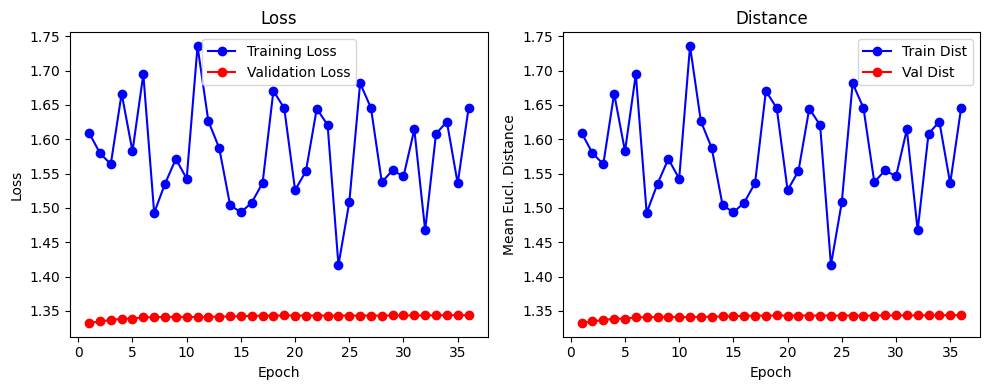
\includegraphics[width=0.8\textwidth]{Imgs/orogin_model.png}
    \caption{Training and validation loss and MED metrics during model training.}
    \label{fig:loss_MED_metrics}
\end{figure}

\subsection{Hyperparameter Tuning}
Hyperparameter optimization was conducted using the \textbf{Hyperband Tuner}, a method that efficiently searches the hyperparameter space by dynamically allocating resources to the most promising configurations. Hyperband evaluates multiple configurations with varying levels of computational resources, discarding less effective configurations early, and focusing resources on the most promising ones.

During the tuning process, several hyperparameters were optimized:
\begin{itemize}
    \item \textbf{Learning rate:} Determines the size of the update step during gradient descent, controlling the speed at which the model learns from the data.
    \item \textbf{Number of units in the dense layers:} Specifies the number of neurons in each fully connected layer, impacting the model's capacity to learn complex features.
    \item \textbf{Dropout rate:} Defines the fraction of neurons to randomly disable during training, reducing the risk of overfitting.
    \item \textbf{Activation functions:} Various activation functions were tested to determine the best-performing option for the dense layers. The following activation functions were included in the tuning:
\end{itemize}

\subsubsection{Activation Functions Used:}
\begin{enumerate}
    \item \textbf{ReLU (Rectified Linear Unit):}
    \[
    f(x) = \max(0, x)
    \]
    ReLU introduces non-linearity by outputting the input directly if it is positive and zero otherwise. It is computationally efficient and mitigates the vanishing gradient problem, making it a popular choice for deep learning models.

    \item \textbf{Tanh (Hyperbolic Tangent):}
    \[
    f(x) = \tanh(x) = \frac{e^x - e^{-x}}{e^x + e^{-x}}
    \]
    The Tanh function outputs values between \(-1\) and \(1\), providing centered activations. This can improve optimization when inputs have negative values, but it is prone to the vanishing gradient problem in deep networks.

    \item \textbf{Leaky ReLU:}
    \[
    f(x) = 
    \begin{cases} 
    x & \text{if } x > 0, \\ 
    \alpha x & \text{if } x \leq 0,
    \end{cases}
    \]
    where \(\alpha\) is a small constant. Leaky ReLU modifies the standard ReLU by allowing a small, non-zero gradient for negative inputs, addressing the "dying ReLU" problem where neurons can become inactive and stop learning.

    \item \textbf{ELU (Exponential Linear Unit):}
    \[
    f(x) = 
    \begin{cases} 
    x & \text{if } x > 0, \\ 
    \alpha (e^x - 1) & \text{if } x \leq 0,
    \end{cases}
    \]
    where \(\alpha\) determines the saturation value for negative inputs. ELU improves upon ReLU by making negative values smoother, speeding up learning and avoiding issues with dead neurons.
\end{enumerate}

\subsubsection{Purpose of Hyperparameter Tuning:}
Hyperparameter tuning is a critical step in optimizing the performance of the model. By systematically searching for the best combination of hyperparameters, the model achieves higher accuracy and generalization. The \textbf{Hyperband Tuner} dynamically allocated resources to configurations involving various activation functions, learning rates, and dropout rates. The best configuration was selected based on the validation performance, with metrics such as loss and Mean Euclidean Distance (MED) guiding the process.

The two best-performing configurations are summarized below:

\begin{table}[H]
\centering
\caption{Top 2 Hyperparameter Tuning Results}
\label{tab:hyperparameter_tuning_results}
\begin{tabular}{|c|c|c|}
\hline
\textbf{Hyperparameter}       & \textbf{Rank 1 Model (Trial 0076)} & \textbf{Rank 2 Model (Trial 0083)} \\ \hline
\textbf{Score (MED)}          & 0.3531                            & 0.3533                            \\ \hline
\textbf{Learning Rate}        & 0.0001917                         & 0.0002445                         \\ \hline
\textbf{Activation Function}  & Tanh                              & ELU                                \\ \hline
\textbf{Units in Layer 1}     & 224                               & 256                               \\ \hline
\textbf{Units in Layer 2}     & 48                                & 64                                \\ \hline
\textbf{Dropout Rate}         & 0.1                               & 0.1                               \\ \hline
\textbf{Leaky ReLU Alpha}     & 0.1                               & 0.1                               \\ \hline
\textbf{Epochs}               & 30                                & 30                                \\ \hline

\end{tabular}
\end{table}



\subsubsection{Analysis of  Hyperparameter Tuning Results}
The two models achieved similar performance, with the second-ranked model (Trial ID: 0083) achieving a slightly lower MED score. The use of different activation functions (\textbf{Tanh} in Rank 1 and \textbf{ELU} in Rank 2) highlights the model's sensitivity to activation choices. Both models used low learning rates (around 0.0002) and a moderate dropout rate of 0.1. A low learning rate helps the model make smaller updates to its parameters, reducing the risk of instability or missing the best solutions. This is especially important for complex models, as large updates can cause the model to jump over good solutions or get stuck in bad ones.

The dropout rate of 0.1 keep a balance between preventing overfitting and keeping enough neurons active for learning. By randomly deactivating 10 of the neurons during training, the model learns stronger and more general features without losing its ability to identify complex patterns.
These results demonstrate the importance of hyperparameter tuning in achieving optimal model configurations for UAV localization.

\subsection{ Validation and Cross-Validation}
To ensure robustness, the model was evaluated using \textbf{K-Fold Cross-Validation}, where the dataset was divided into \(k = 10\) subsets. In this process, each subset was used as a validation set while the remaining subsets were used for training. This approach provided a comprehensive evaluation of the model's performance across multiple data splits, ensuring that the results were not biased by a particular partition of the data.
\begin{itemize}
    \item \textbf{First Ranked Model:} Achieved an average loss of \(0.3654\) and an average MED of \(0.3654\) across all folds. 
    \item \textbf{Second Ranked Model:} Achieved an average loss of \(0.3369\) and an average MED of \(0.3369\) across all folds. 
\end{itemize}
The training process for each fold was monitored, and the loss was recorded epoch-by-epoch. The two best-performing models were evaluated separately, and their loss improvement trends across all folds are illustrated in Figure~\ref{fig:folds_best_model} and Figure~\ref{fig:folds_second_best_model}.



\begin{figure}[H]
    \centering
    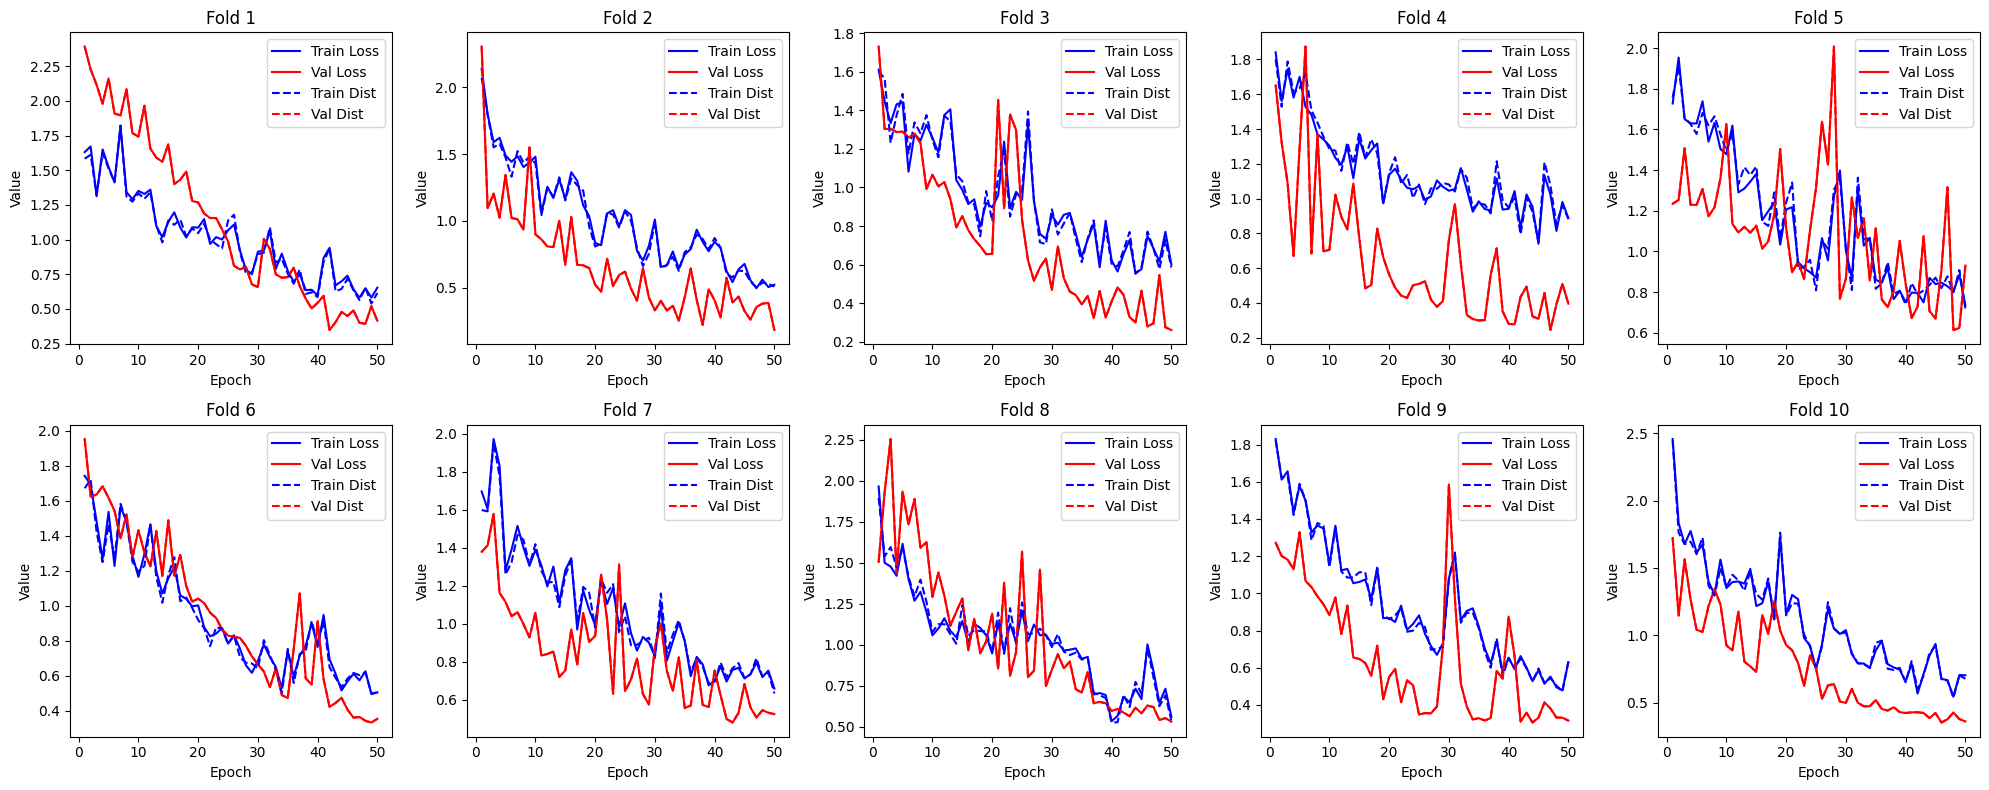
\includegraphics[width=0.9\textwidth]{Imgs/best_model_out.png}
    \caption{Epoch-by-epoch loss improvement for the first rank model during 10-fold cross-validation.}
    \label{fig:folds_best_model}
\end{figure}

\begin{figure}[H]
    \centering
    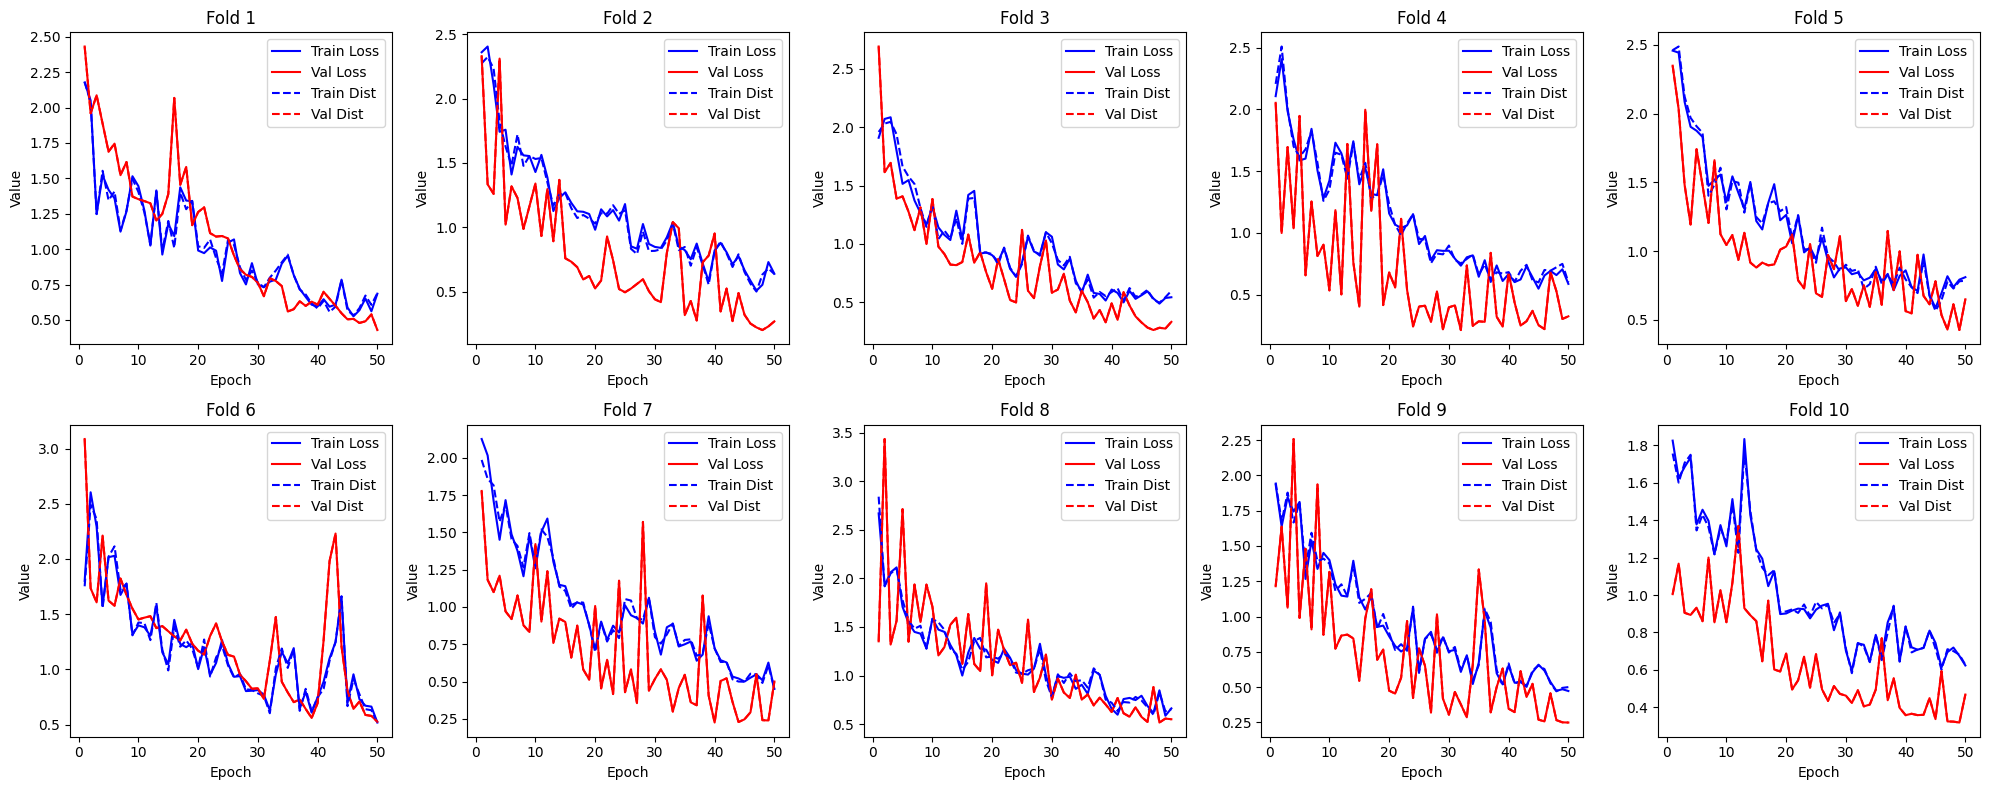
\includegraphics[width=0.9\textwidth]{Imgs/second_best_out.png}
    \caption{Epoch-by-epoch loss improvement for the second rank model during 10-fold cross-validation.}
    \label{fig:folds_second_best_model}
\end{figure}

\subsection{Output and Deployment}
The trained model predicts the UAV’s final location based on input trajectory images and initial 
relative position. The model is saved in \texttt{.keras} format and can be reloaded for deployment. This ensures its utility in real-time UAV localization tasks.

This architecture combines state-of-the-art image processing (CNN) with numerical data fusion to predict UAV locations. A schematic representation of the model is shown in Figure~\ref{fig:model_architecture}.

\begin{figure}[H]
    \centering
    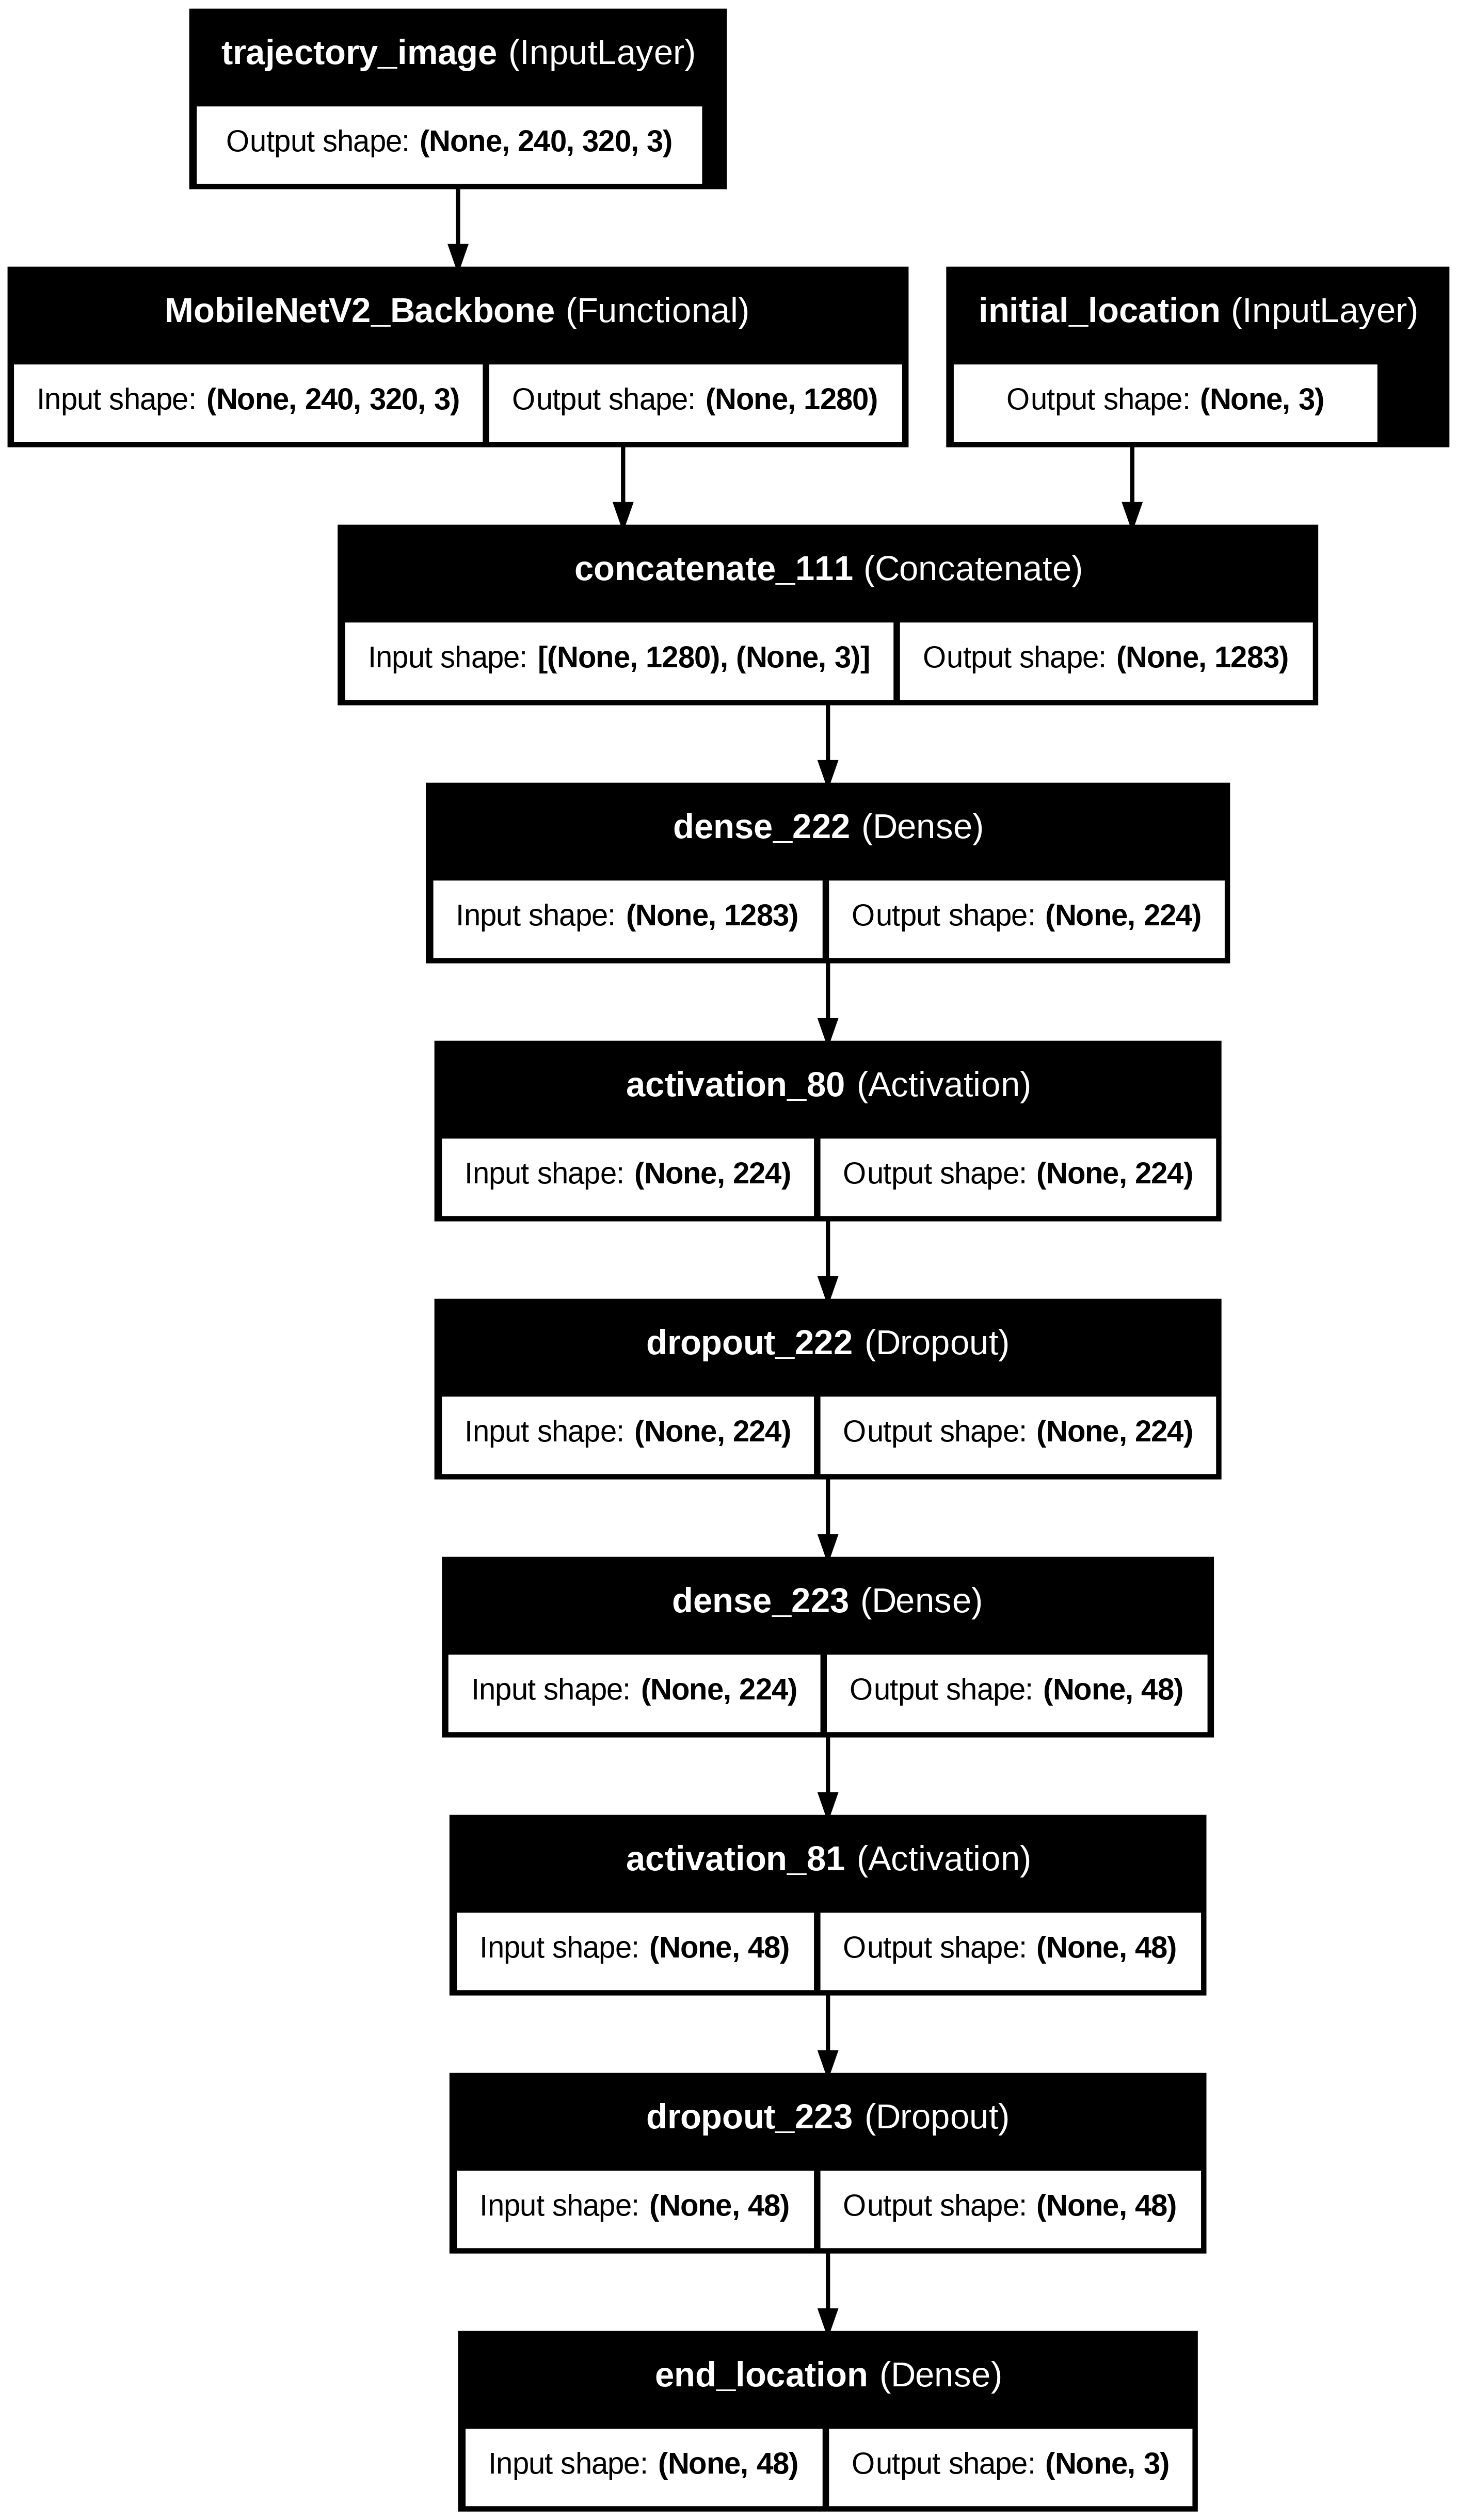
\includegraphics[width=0.5\textwidth]{Imgs/cnn.png}
    \caption{Schematic representation of the proposed model architecture.}
    \label{fig:model_architecture}
\end{figure}


\section{Running the Model in Simulation}

The model deployment in the simulation environment involves replicating the complete data processing pipeline, starting from trajectory image collection to final prediction.

\begin{itemize}
    \item Collect the pose data and camera images while target UAV executing its trajectory.
    \item The observer UAV camera images were preprocessed to extract the target UAV's trajectory image.
    \item Using processed data, make prediciton and send the predicted values to GUI.
\end{itemize}

The model demonstrated strong performance in the simulation environment, accurately predicting the target UAV's position under various noise levels and trajectory types. The integration of the preprocessing pipeline ensured that the model input formatted correctly. Figure~\ref{fig:prediction_vs_real} illustrates the comparison between the predicted and real positions of the UAV, with numbered points representing corresponding predictions and actual positions. Noise levels and error metrics for each point are provided in the Table~\ref{table:noise_levels_errors_locations}

\begin{figure}[h!]
    \centering
    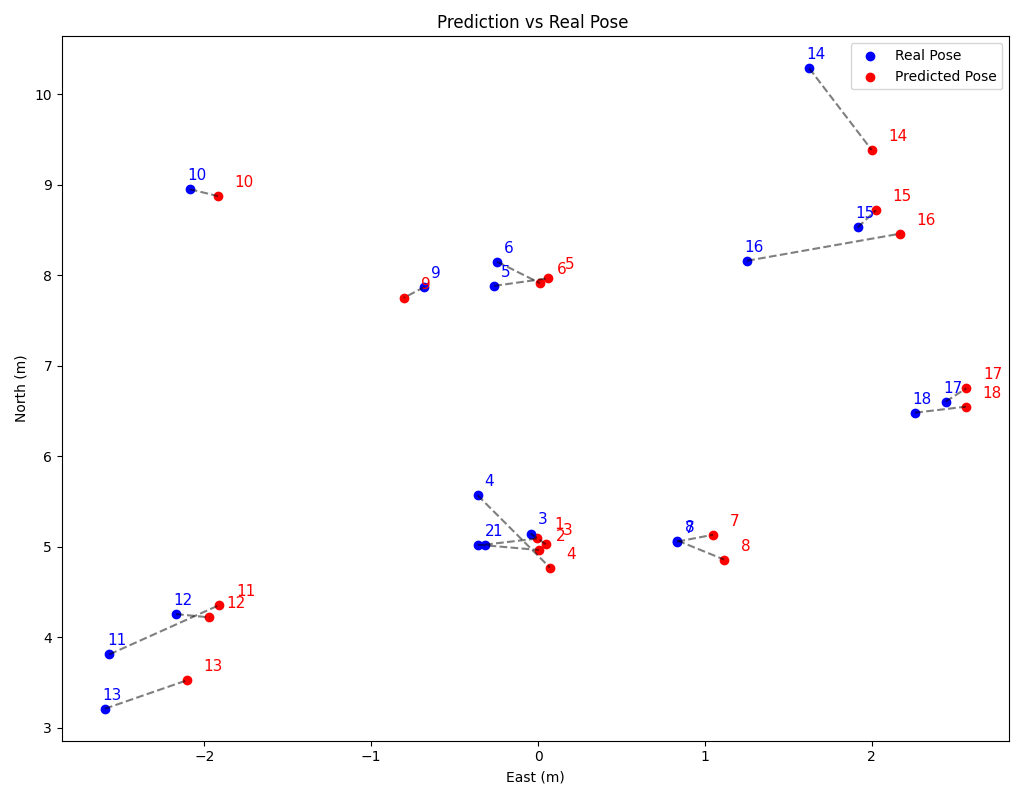
\includegraphics[width=0.8\textwidth]{Imgs/results.png} % Replace with the path to your graph image
    \caption{Comparison of predicted and real UAV positions. Points are numbered for reference, and noise levels and errors are detailed in the Table~\ref{table:noise_levels_errors_locations}.}
    \label{fig:prediction_vs_real}
\end{figure}

\par The results show that the model performs well, with errors typically ranging between 0.2 and 0.4 meters under low to medium noise levels. For example, when the noise is low (e.g., observer UAV noise level: 2.0, target UAV noise level: 3.0), the error often stays below 0.4. However, as the noise levels increase (e.g., target UAV noise level = 10.0 or 11.0), the errors grow, sometimes exceeding 0.9 meters. This indicates that while the model can handle mild to moderate noise effectively, its performance declines with higher noise levels.

\begin{table}[h!]
\centering
\caption{Noise Levels, Errors, and UAV Locations}
\label{table:noise_levels_errors_locations}
\resizebox{\textwidth}{!}{%
\begin{tabular}{|c|c|c|c|c|c|}
\hline
\textbf{Point} & \textbf{Observer UAV (NED (m))} & \textbf{Target UAV (NED (m))} & \textbf{Observer UAV oise Level} & \textbf{Target UAV Noise Level} & \textbf{Error (m)} \\ \hline
1 & 0.092, -0.059, 20.006 & 5.078, -0.036, 20.040 & 2.0 & 3.0 & 0.3614 \\ \hline
2 & 0.035, 0.108, 19.996 & 4.955, -0.327, 20.120 & 2.0 & 5.0 & 0.3865 \\ \hline
3 & -0.041, 0.008, 19.988 & 4.933, -0.263, 20.160 & 2.0 & 8.0 & 0.1608 \\ \hline
4 & 0.086, -0.044, 20.008 & 4.844, -0.454, 20.210 & 2.0 & 10.0 & 0.9115 \\ \hline
5 & 0.068, -0.033, 19.995 & 8.072, -0.236, 20.050 & 2.0 & 5.0 & 0.3527 \\ \hline
6 & 0.005, 0.030, 20.013 & 7.894, -0.091, 20.050 & 2.0 & 8.0 & 0.3784 \\ \hline
7 & 0.024, 1.032, 20.001 & 5.145, 1.062, 20.050 & 0.0 & 0.0 & 0.4219 \\ \hline
8 & 0.022, 1.058, 19.990 & 4.822, 1.117, 20.070 & 2.0 & 5.0 & 0.3839 \\ \hline
9 & -0.021, -0.991, 20.009 & 7.861, -1.008, 20.020 & 2.0 & 7.0 & 0.1731 \\ \hline
10 & -0.093, -2.024, 19.992 & 9.375, -2.224, 20.090 & 2.0 & 10.0 & 0.2553 \\ \hline
11 & 0.005, -2.109, 20.022 & 4.121, -1.589, 19.890 & 2.0 & 7.0 & 0.9544 \\ \hline
12 & -0.015, -2.001, 19.978 & 3.865, -2.142, 19.940 & 2.0 & 7.0 & 0.5237 \\ \hline
13 & 0.088, -2.041, 20.022 & 2.840, -2.070, 19.910 & 2.0 & 6.0 & 0.9168 \\ \hline
14 & 0.041, 1.970, 20.004 & 9.865, 2.142, 19.910 & 2.0 & 4.0 & 0.9774 \\ \hline
15 & 0.104, 1.903, 20.018 & 8.996, 1.970, 19.940 & 2.0 & 7.0 & 0.2368 \\ \hline
16 & 0.026, 1.929, 19.998 & 8.451, 1.543, 19.940 & 2.0 & 11.0 & 0.9642 \\ \hline
17 & -0.031, 2.457, 20.007 & 6.692, 2.315, 19.890 & 2.0 & 6.0 & 0.3754 \\ \hline
18 & 0.015, 2.521, 19.991 & 6.525, 2.506, 19.930 & 0.0 & 0.0 & 0.4241 \\ \hline
\end{tabular}%    

}
\small
\textbf{Observer UAV (NED (m))}: The starting position of the observer UAV in North-East-Down (NED) coordinates, measured in meters. \\
\textbf{Target UAV (NED (m))}: The starting position of the target UAV in North-East-Down (NED) coordinates, measured in meters. \\
\textbf{Observer UAV Noise Level}: The level of GPS noise applied to the observer UAV's position during simulation. \\
\textbf{Target UAV Noise Level}: The level of GPS noise applied to the target UAV's position during simulation. \\
\textbf{Error (m)}: The Euclidean distance (in meters) between the predicted and actual positions of the target UAV.

\end{table}


\begin{figure}[h!]
    \centering
    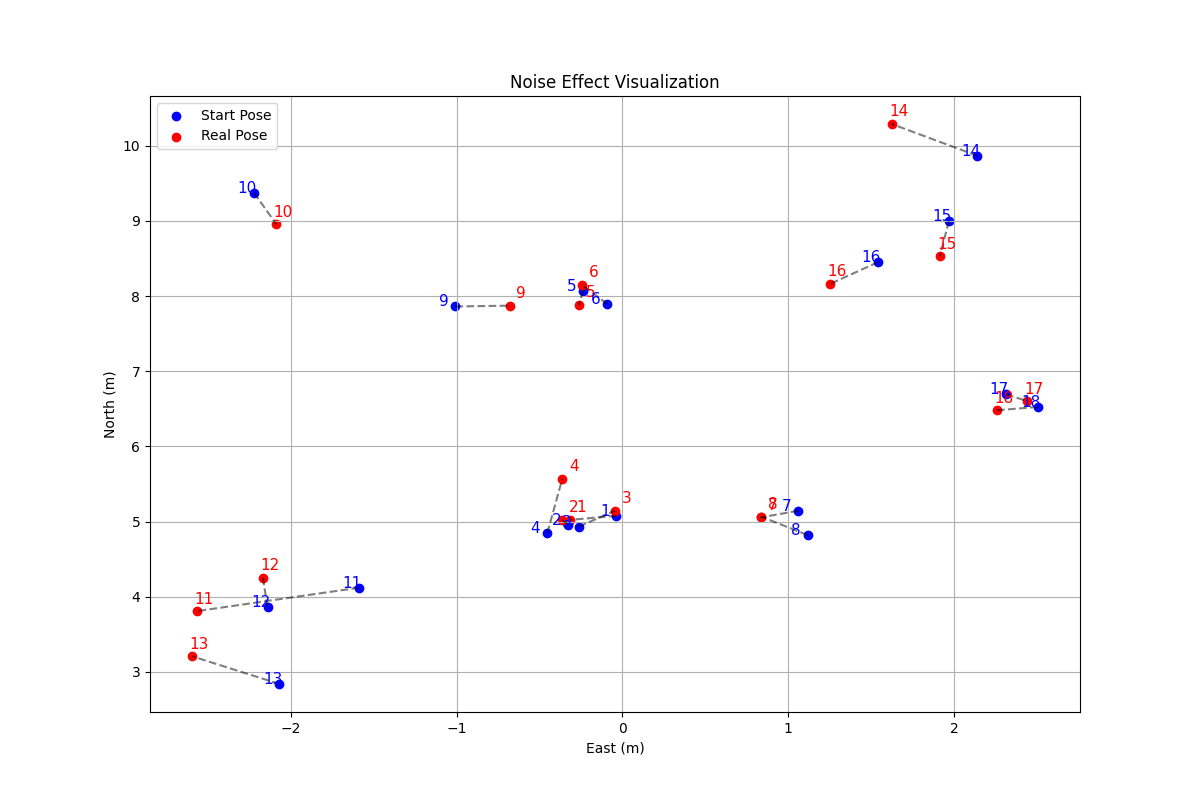
\includegraphics[width=0.8\textwidth]{Imgs/noise_effect.png} % Replace with the path to your graph image
    \caption{Effect of Noise on End Location of Target UAV}
\label{fig:noise_effect_target_UAV}
\end{figure}

\par When looking at individual axes, errors in the East axes contribute significantly to the overall error. For instance, the predicted North axes values often deviate slightly from the real values, which can accumulate into a larger total error. In addition, some starting poses—especially those with more negative North values or higher absolute East values—lead to larger errors. This suggests that the model could improve with additional training data in these specific areas.



The Figure~\ref{fig:noise_effect_target_UAV} displays how GPS noise in the system causes variations in the target UAV’s final position. The red points represent target UAV's trajectories last positions, the blue points represent the measured target UAV's trajectories last positions. 
In summary, the model can predict relative positions  with errors generally between 0.2 and 0.4 meters. However, higher noise levels reduce its accuracy. The model achieved an average error distance of 0.51 meter between the predicted and actual
positions.

\chapter{Conclusions}
The project has demonstrated that the final position of the target UAV can be successfully estimated using its trajectory and starting position, even in environments with GPS noise. The CNN model, developed and tested in a simulation environment, achieved an average error distance of 0.51 meter between the predicted and actual positions, meeting the project’s success criteria.

The model’s architecture and performance indicate that it can be further enhanced and tested under different scenarios by incorporating additional training data. This project has validated the feasibility of location estimation in noisy GPS environments by minimizing the reliance on extensive flight data from the target UAV.



% DON'T INPUT FILES AFTER HERE
\begin{outertitles}
\clearpage
\setlength{\emergencystretch}{1em}
\printbibliography
\addtocontents{toc}{\protect\vspace{18pt}}
\addcontentsline{toc}{chapter}{Bibliography}
%% If you don't want a CV or appendices add a % at the beginning of the relevant line

\end{outertitles}
\end{document}